\documentclass[12pt,a4paper]{article}
\usepackage[czech]{babel}
\usepackage[utf8]{inputenc} 
\usepackage{listings}
\lstset{language=C}
\usepackage{minted}
\usepackage[hidelinks]{hyperref}
\usepackage{graphicx}
\usepackage{caption}
\usepackage[all]{hypcap}
\usepackage{pdfpages}

\newcommand{\Csh}{C\#}

\renewcommand\listingscaption{Výpis}


\begin{document}
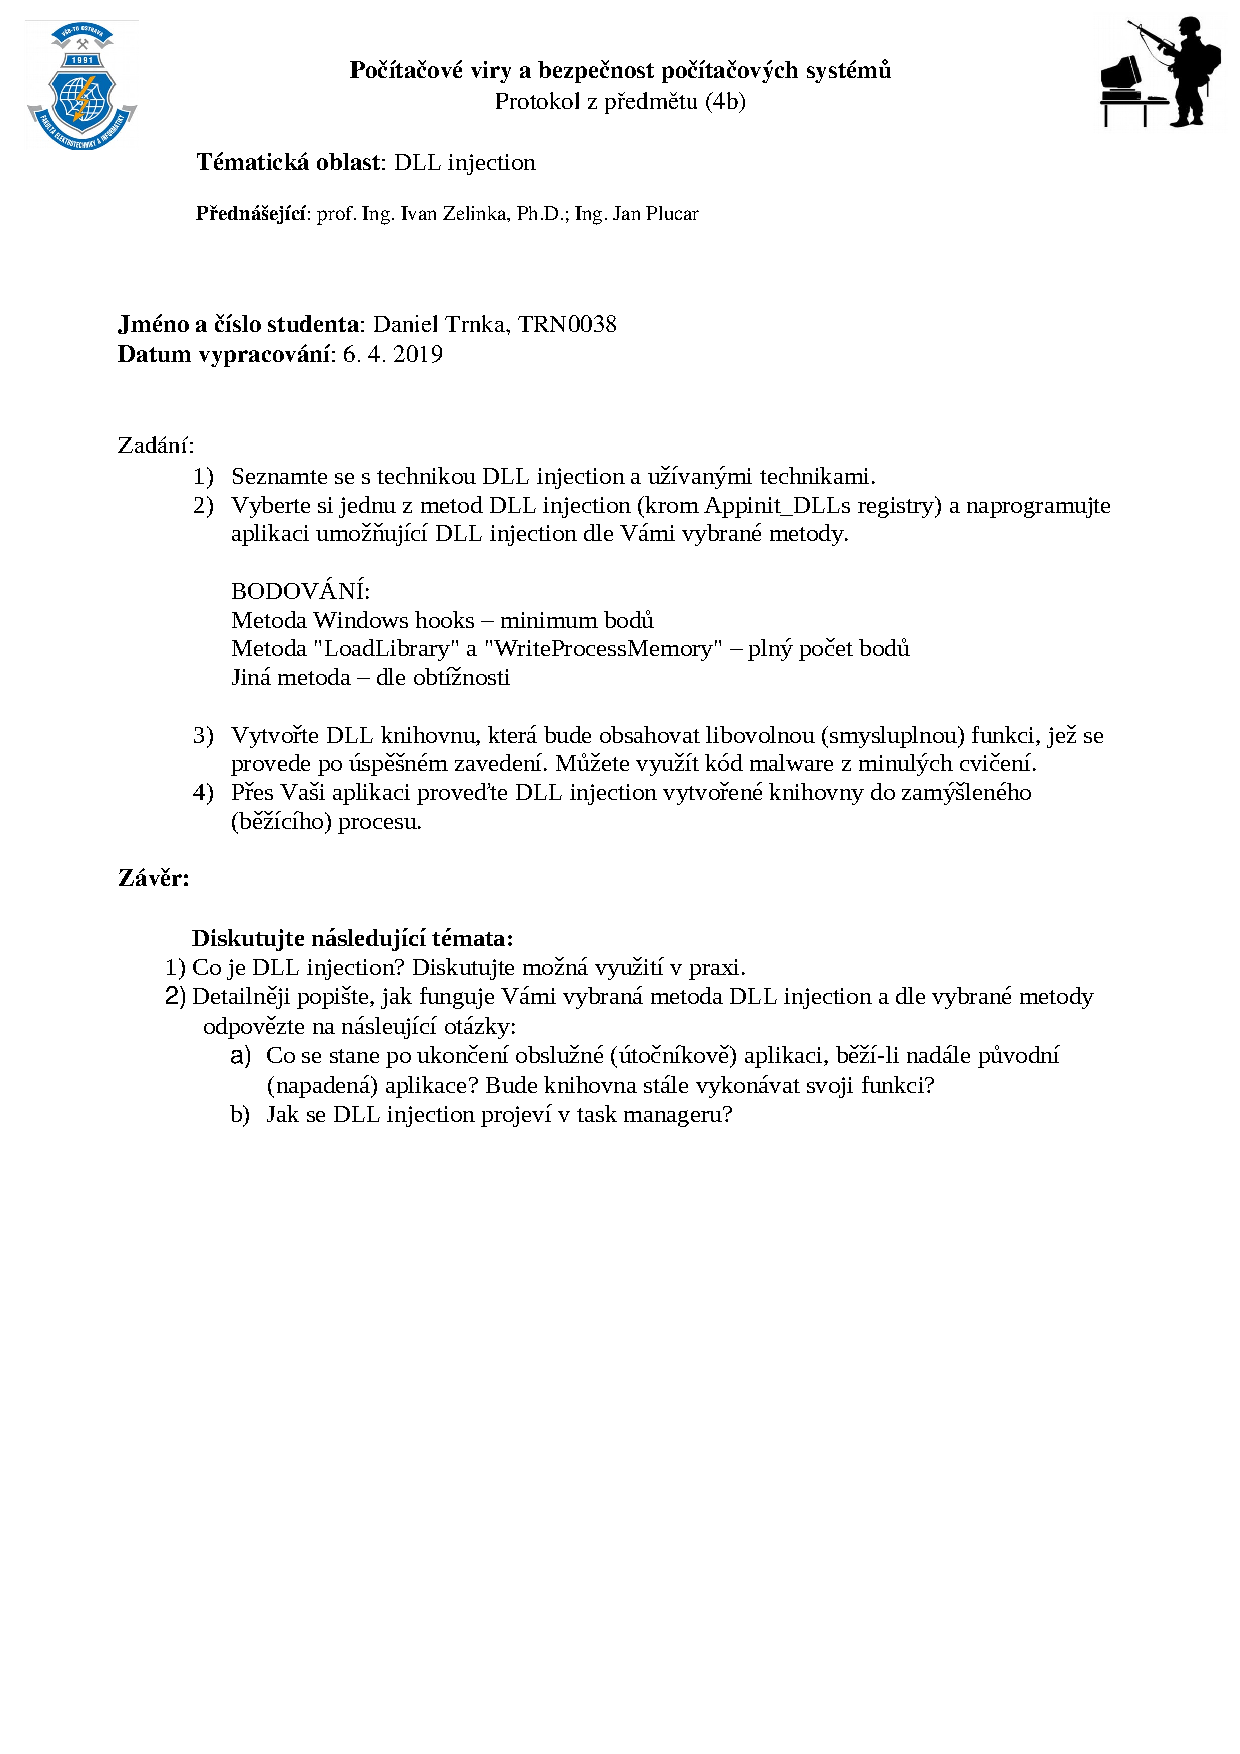
\includepdf[pages=1]{zadani.pdf}

\section{Zadání}
\subsection{Techniky DLL injection}
DLL injection umožňuje vložit do jiného legitimního procesu dynamickou knihovnu a vykonávat ji pod daným procesem.
Lze tak skrýt případný malware.

Existuje několik možnosti jak provést DLL injection:



\begin{description}
\item[] 
\footnote{\url{https://resources.infosecinstitute.com/using-setwindowshookex-for-dll-injection-on-windows/}}	
	
	
	
\item[Appinit\_DLL] injektuje DLL nastavenou v registrech do všech procesů využívající knihovnu \texttt{user32.dll}. 
Nastavení musí provést administrátor a systém se musí zavést s vypnutým SecureBoot.
\end{description}

\subsection{DLL injection pomocí \texttt{LoadLibrary} a \texttt{WriteProcessMemory}}
Windows API umožňuje pomocí funkce \texttt{CreateRemoteThread} spustit vlákno v jiném procesu.
Pro spuštění vlákna potřebujeme \texttt{HANDLE} na daný proces a adresu funkce či obecně první instrukce.
Dále je možné do této funkce předat jediný číselný argument.

V adresáři \texttt{c/function\_call} je ukázka, jak z \texttt{inject.c} zavolat funkci v \texttt{victim.c}.
Programy je nutné zkompilovat pomocí překladače \texttt{x86\_64-w64-mingw32-gcc} či v překladači MSVCC s vypnutou volbou \texttt{/DYNAMICBASE}.
V opačném případě se obraz procesu nahrává na náhodnou adresu v rámci adresního prostoru procesu, aby se zkomplikovali možné útoky, kdy například útočník zná adresu funkce.
V rámci ukázek se volá funkce bez parametru, s číselný parametrem, ale také se předává ukazatel na pole či se volá funkce s více parametry.

Pro předání pole do funkce je nutné v cizím procesu alokovat pole potřebné velikosti a překopírovat sem obsah.
Poté se ve funkci \texttt{CreateRemoteThread} předá jako první parametr adresa alokované paměti v cizím procesu.

Zavolání funkce s více parametry vyžaduje do procesu vložit instrukce.
Konvence pro předávání argumentu na x86\_64 vyžaduje, aby první čtyři parametry byly předány pomocí registrů \texttt{RCX}, \texttt{RDX}, \texttt{R8} a \texttt{R9}\footnote{\url{https://en.wikipedia.org/wiki/X86_calling_conventions\#Microsoft_x64_calling_convention}}.
Pro zavolání funkce se třemi číselnými argumenty \texttt{1}, \texttt{2} a \texttt{3} je nutné vložit instrukce, které do registrů vloží hodnoty.
Protože funkce vyžaduje 3x \texttt{int}, tak je možné provést zápis argumentů do 32bitových registrů, čímž se získá kratší opcodes.
Zavolání funkce se pak provede skokem na absolutní adresu.
Instrukce skoku \texttt{jmp} neumožňuje provést skok na 64bitovou adresu a je tedy nutné tuto adresu uložit do registru a následně provést skok na hodnotu uloženou v registru: 

\begin{minted}{asm}
mov ecx, 1
mov edx, 2
mov r8d, 3
mov rax, remote_add
jmp rax
\end{minted}

Binární reprezentaci instrukci lze manuálně získat například pomocí online nástroje\footnote{\url{https://defuse.ca/online-x86-assembler.htm}}.
Tuto reprezentaci je nutné vložit do alokované paměti v cizím procesu a následně zavolat \texttt{CreateRemoteThread} s adresou na dané instrukce.
Vlákno provede nastavení registrů a skok do funkce \texttt{add}, která vytiskne argumenty a jejich součet vrátí.
Vrácení hodnoty \texttt{int} probíhá pomocí registru \texttt{EAX}.
Protože se tato funkce volala pomocí skoku \texttt{jmp}, tak se jedná o funkci po jejímž návratu je vlákno ukončeno a návratová hodnota je předana předkovi jako \texttt{EXIT CODE}.

Nahrání DLL do procesu je možné pomocí funkce: \mint{c}{void* LoadLibraryA(char* path)}
Funkce vyžaduje jediný argument a to řetězec obsahující cestu k dynamické knihovně.
Jedinou komplikaci je, že argumentem je řetězec a je tedy nutné v cizím procesu alokovat paměť pro tento řetězec.
Další komplikaci by mohlo být získání adresy funkce \texttt{LoadLibraryA}.
Tato funkce je ale součástí knihovny \texttt{kernel32.dll}, která je do všech procesů namapovaná na stejné místo.
Tento problém tedy odpadá.

Při načtení dynamické knihovny se zavolá funkce \texttt{DllMain} z dané knihovny.
Pokud funkce vrátí \texttt{1}, tak se vlákno s funkci \texttt{LoadLibraryA} ukončí a předek může získat adresu načtené knihovny z \texttt{EXIT CODE}.
Pro zavolání vlastní funkce v dynamické knihovně je nutné k této adrese přičíst offset od začátku knihovny.

\subsection{DLL knihovna}
Dynamická knihovna \texttt{c/inject\_dll/powershell.c} definuje dvě funkce.
První funkce \texttt{DllMain} se zavolá při načtení/odebrání knihovny do procesu a vypíše PID daného procesu.
Druhá funkce \texttt{run} vytvoří nový PowerShell proces a vykoná zakódovaný BASE64 kód z minulého cvičení.


\subsection{Injection}
Program \texttt{c/inject/inject.c} provádí výše popsaný postup DLL injection.

Pro vložení DLL do procesu \texttt{cmd.exe} lze zavolat:
\begin{minted}{bash}
$ inject.exe cmd.exe E:/5/c/inject_dll/powershell.dll
\end{minted}

\section{Závěr}
\begin{enumerate}
	\item 
\end{enumerate}

\end{document}